\documentclass[10pt,leqno]{article}

\usepackage[%
  tmargin=1.2in,bmargin=1.2in,%
  lmargin=1.8in,rmargin=1.8in,%
]{geometry}
\usepackage{fancyhdr}
\usepackage{titlesec}
\usepackage{appendix}
\usepackage{microtype}
\usepackage[hyphens]{url}
\usepackage{enumitem}
\usepackage{xspace}
\usepackage{etoolbox}
\usepackage{ifthen}
\usepackage{tikz}
\usepackage{tikz-cd}

\usepackage{amsmath}
\definecolor{darkred}{rgb}{0.5,0.0,0.0}
\usepackage[%
  colorlinks,%
  linkcolor=darkred,%
  citecolor=darkred,%
  urlcolor=darkred,%
]{hyperref}
\usepackage{amsthm,amssymb}
% \usepackage[lining,semibold]{libertine}
% \usepackage{textcomp,stmaryrd}
% \usepackage[libertine,cmintegrals,bigdelims]{newtxmath}
% \useosf
% \usepackage[%
%   cal=boondox, calscaled=0.97,%
%   bb=boondox, bbscaled=0.98,%
% ]{mathalfa}
\usepackage{cleveref}

\frenchspacing
\urlstyle{rm}

\AtBeginDocument{%
  \setlength{\abovedisplayskip}{1.5ex plus 0.3ex minus 0.3ex}%
  \setlength{\abovedisplayshortskip}{1.0ex plus 0.3ex minus 0.3ex}%
  \setlength{\belowdisplayskip}{1.5ex plus 0.3ex minus 0.3ex}%
  \setlength{\belowdisplayshortskip}{1.0ex plus 0.3ex minus 0.3ex}%
}

\let\theoldbibliography\thebibliography
\renewcommand{\thebibliography}[1]{%
  \theoldbibliography{#1}%
  \setlength{\parskip}{0ex}
  \setlength{\itemsep}{0.5ex plus 0.2ex minus 0.2ex}
  \small
}

\pagestyle{fancy}
\renewcommand{\headrulewidth}{0pt}
\renewcommand{\footrulewidth}{0pt}
\fancyhf{}
\fancyfoot[C]{\small\thepage}

\renewcommand{\title}[1]{\newcommand{\thetitle}{#1}}
\renewcommand{\author}[1]{\newcommand{\theauthor}{#1}}
\renewcommand{\date}[1]{\newcommand{\thedate}{#1}}

\renewcommand{\maketitle}{%
  \begin{center}
    {\bfseries\MakeUppercase{%
      \thetitle}}\\[2.5ex]
    {\footnotesize\MakeUppercase{%
      \theauthor}}\\[2.5ex]
    \ifthenelse{\equal{\thedate}{}}{}{%
      \small%
      \setlength{\tabcolsep}{0.2em}%
      \begin{tabular}{rl}
        original: & \thedate \\
        updated: & \today
      \end{tabular}
    }
  \end{center}
  \vspace{2.5ex}
  \thispagestyle{fancy}
}

%%%%%%%%%%%%%%%%%%%%%%%%%%%%%%%%%%%%%%%%%%%%%%%%%%%%%%%%%%%%%%%%%%%%%%

\cspreto{section}{\setcounter{equation}{0}}

\titleformat{\section}{\centering\scshape}{\thesection.}{0.4em}{}
\titlespacing{\section}{0pt}{*4}{*1}
\titleformat{\subsection}{\scshape}{\thesubsection.}{0.4em}{}
\titlespacing{\subsection}{0pt}{*2.5}{*1}

% Display format for equations
\newcommand{\crefeqfmt}[1]{
  \crefformat{#1}{(##2##1##3)}
  \Crefformat{#1}{(##2##1##3)}
  \crefrangeformat{#1}{(##3##1##4--##5##2##6)}
  \Crefrangeformat{#1}{(##3##1##4--##5##2##6)}
  \crefmultiformat{#1}{(##2##1##3}{, ##2##1##3)}{, ##2##1##3}{, ##2##1##3)}
  \Crefmultiformat{#1}{(##2##1##3}{, ##2##1##3)}{, ##2##1##3}{, ##2##1##3)}
  \crefrangemultiformat{#1}{(##3##1##4--##5##2##6}{, ##3##1##4--##5##2##6)}{, ##3##1##4--##5##2##6}{, ##3##1##4--##5##2##6)}
  \Crefrangemultiformat{#1}{(##3##1##4--##5##2##6}{, ##3##1##4--##5##2##6)}{, ##3##1##4--##5##2##6}{, ##3##1##4--##5##2##6)}
}
% Display format for sections
\newcommand{\crefsecfmt}[1]{%
  \crefformat{#1}{\S##2##1##3}
  \Crefformat{#1}{\S##2##1##3}
  \crefrangeformat{#1}{\S\S##3##1##4--##5##2##6}
  \Crefrangeformat{#1}{\S\S##3##1##4--##5##2##6}
  \crefmultiformat{#1}{\S\S##2##1##3}{ and~##2##1##3}{, ##2##1##3}{ and~##2##1##3}
  \Crefmultiformat{#1}{\S\S##2##1##3}{ and~##2##1##3}{, ##2##1##3}{ and~##2##1##3}
  \crefrangemultiformat{#1}{\S\S##3##1##4--##5##2##6}{ and~##3##1##4--##5##2##6}{, ##3##1##4--##5##2##6}{ and~##3##1##4--##5##2##6}
  \Crefrangemultiformat{#1}{\S\S##3##1##4--##5##2##6}{ and~##3##1##4--##5##2##6}{, ##3##1##4--##5##2##6}{ and~##3##1##4--##5##2##6}
}
\crefeqfmt{equation}
\crefeqfmt{enumi}
\crefeqfmt{enumii}
\crefsecfmt{section}
\crefsecfmt{subsection}
\crefsecfmt{appendix}
\crefname{part}{Part}{Parts}
\crefname{chapter}{Chapter}{Chapters}
\crefname{figure}{Figure}{Figures}

\makeatletter

\newcommand{\thmnumfont}{\bfseries}
\newcommand{\thmheadfont}{\bfseries}
\newcommand{\thmnotefont}{\bfseries}
\newcommand{\thmhorizspace}{0.4em}

\def\swappedhead#1#2#3{%
  \thmnumber{\@upn{{\thmnumfont#2}}\@ifnotempty{#1}{.\hspace{0.25em}}}%
  \thmheadfont\thmname{#1}%
  \@ifnotempty{#3}{\ \thmnote{\thmnotefont(#3)}}%
}
\swapnumbers

\newtheoremstyle{block}%
  {2.0ex plus 0.2ex minus 0.1ex}% Space above
  {2.0ex plus 0.2ex minus 0.1ex}% Space below
  {} % Body font
  {} % Indent amount
  {\thmheadfont} % Theorem head font
  {.} % Punctuation after theorem head
  {\thmhorizspace} % Space after theorem head
  {} % Theorem head spec (can be left empty, meaning ‘normal’)

\renewenvironment{proof}[1][Proof]{\par
  \pushQED{\qed}%
  \normalfont%
  \topsep1ex plus 0.2ex minus 0.1ex\relax%
  \labelsep \thmhorizspace\relax%
  \trivlist
  \item[\hskip\labelsep\thmheadfont
    #1\@addpunct{.}]\ignorespaces
}{%
  \popQED\endtrivlist\@endpefalse%
}

\makeatother

\theoremstyle{block}

\newcommand{\defthm}[2]{%
  \newtheorem{#1}[equation]{#2}%
  \crefeqfmt{#1}%
  \newtheorem*{#1*}{#2}%
}

\defthm{algorithm}{Algorithm}
\defthm{conjecture}{Conjecture}
\defthm{construction}{Construction}
\defthm{convention}{Convention}
\defthm{corollary}{Corollary}
\defthm{definition}{Definition}
\defthm{definitions}{Definitions}
\defthm{example}{Example}
\defthm{examples}{Examples}
\defthm{exercise}{Exercise}
\defthm{fact}{Fact}
\defthm{intuition}{Intuition}
\defthm{lemma}{Lemma}
\defthm{notation}{Notation}
\defthm{nothing}{}
\defthm{proposition}{Proposition}
\defthm{question}{Question}
\defthm{remark}{Remark}
\defthm{remarks}{Remarks}
\defthm{situtation}{Situation}
\defthm{theorem}{Theorem}

\setlist{%
  leftmargin=2.5em, parsep=0ex, listparindent=\parindent,
  itemsep=1.0ex, topsep=1.0ex,%
}

\setlist[enumerate, 1]{%
  label=(\alph*),%
  ref=\alph*,%
  widest=d,%
}
\setlist[enumerate, 2]{%
  label=(\roman*),%
  ref=\theenumi.\roman*,%
}
\setlist[itemize, 1]{%
  label=$\vcenter{\hbox{\footnotesize$\bullet$}}$,%
}
\setlist[itemize, 2]{label=--}

%%%%%%%%%%%%%%%%%%%%%%%%%%%%%%%%%%%%%%%%%%%%%%%%%%%%%%%%%%%%%%%%%%%%%%

\makeatletter

\let\ea\expandafter

\newcount\foreachcount

\def\foreachletter#1#2#3{\foreachcount=#1
  \ea\loop\ea\ea\ea#3\@alph\foreachcount
  \advance\foreachcount by 1
  \ifnum\foreachcount<#2\repeat}

\def\foreachLetter#1#2#3{\foreachcount=#1
  \ea\loop\ea\ea\ea#3\@Alph\foreachcount
  \advance\foreachcount by 1
  \ifnum\foreachcount<#2\repeat}

% Roman: \rA is \mathrm{A}
\def\definerm#1{%
  \ea\gdef\csname r#1\endcsname{\ensuremath{\mathrm{#1}}\xspace}}
\foreachLetter{1}{27}{\definerm}
\foreachletter{1}{27}{\definerm}
% Script: \sA is \mathscr{A}
\def\definescr#1{%
  \ea\gdef\csname s#1\endcsname{\ensuremath{\mathscr{#1}}\xspace}}
\foreachLetter{1}{27}{\definescr}
% Calligraphic: \cA is \mathcal{A}
\def\definecal#1{%
  \ea\gdef\csname c#1\endcsname{\ensuremath{\mathcal{#1}}\xspace}}
\foreachLetter{1}{27}{\definecal}
% Bold: \bA is \mathbf{A}
\def\definebold#1{%
  \ea\gdef\csname b#1\endcsname{\ensuremath{\mathbf{#1}}\xspace}}
\foreachLetter{1}{27}{\definebold}
% Blackboard Bold: \lA is \mathbb{A}
\def\definebb#1{%
  \ea\gdef\csname l#1\endcsname{\ensuremath{\mathbb{#1}}\xspace}}
\foreachLetter{1}{27}{\definebb}
% Fraktur: \ka is \mathfrak{a}, \kA is \mathfrak{A}
\def\definefrak#1{%
  \ea\gdef\csname k#1\endcsname{\ensuremath{\mathfrak{#1}}\xspace}}
\foreachletter{1}{27}{\definefrak}
\foreachLetter{1}{27}{\definefrak}
% Sans serif: \iA \is \mathsf{A}
\def\definesf#1{%
  \ea\gdef\csname i#1\endcsname{\ensuremath{\mathsf{#1}}\xspace}}
\foreachletter{1}{6}{\definesf}
\foreachletter{7}{14}{\definesf}
\foreachletter{15}{27}{\definesf}
\foreachLetter{1}{27}{\definesf}
% Bar: \Abar is \overline{A}, \abar is \overline{a}
\def\definebar#1{%
  \ea\gdef\csname #1bar\endcsname{\ensuremath{\overline{#1}}\xspace}}
\foreachLetter{1}{27}{\definebar}
\foreachletter{1}{8}{\definebar} % \hbar is something else!
\foreachletter{9}{15}{\definebar} % \obar is something else!
\foreachletter{16}{27}{\definebar}
% Tilde: \Atil is \widetilde{A}, \atil is \widetilde{a}
\def\definetil#1{%
  \ea\gdef\csname #1til\endcsname{\ensuremath{\widetilde{#1}}\xspace}}
\foreachLetter{1}{27}{\definetil}
\foreachletter{1}{27}{\definetil}
% Hats: \Ahat is \widehat{A}, \ahat is \widehat{a}
\def\definehat#1{%
  \ea\gdef\csname #1hat\endcsname{\ensuremath{\widehat{#1}}\xspace}}
\foreachLetter{1}{27}{\definehat}
\foreachletter{1}{27}{\definehat}
% Checks: \Achk is \widecheck{A}, \achk is \widecheck{a}
\def\definechk#1{%
  \ea\gdef\csname #1chk\endcsname{\ensuremath{\widecheck{#1}}\xspace}}
\foreachLetter{1}{27}{\definechk}
\foreachletter{1}{27}{\definechk}
% Underline: \Aund is \underline{A}, \aund is \underline{a}
\def\defineul#1{%
  \ea\gdef\csname #1und\endcsname{\ensuremath{\underline{#1}}\xspace}}
\foreachLetter{1}{27}{\defineul}
\foreachletter{1}{27}{\defineul}

\makeatother

%%%%%%%%%%%%%%%%%%%%%%%%%%%%%%%%%%%%%%%%%%%%%%%%%%%%%%%%%%%%%%%%%%%%%%

\usetikzlibrary{calc,decorations.pathmorphing,shapes,arrows}
\tikzcdset{
  arrow style=tikz,
  diagrams={>={stealth}},
}

\newcommand{\arrlen}{1em}
\renewcommand{\to}{\mathrel{\tikz[baseline]%
    \draw[>=stealth,->](0,0.5ex)--(\arrlen,0.5ex);}}
\newcommand{\from}{\mathrel{\tikz[baseline]%
    \draw[>=stealth,<-](0,0.5ex)--(\arrlen,0.5ex);}}
\renewcommand{\mapsto}{\mathrel{\tikz[baseline]%
    \draw[>=stealth,|->](0,0.5ex)--(\arrlen,0.5ex);}}
\newcommand{\inj}{\mathrel{\tikz[baseline]%
    \draw[>=stealth,right hook->](0,0.5ex)--(\arrlen,0.5ex);}}
\newcommand{\surj}{\mathrel{\tikz[baseline]%
    \draw[>=stealth,->>](0,0.5ex)--(\arrlen,0.5ex);}}
\newcommand{\fromto}{\mathrel{%
  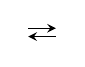
\begin{tikzpicture}[baseline]%
    \draw[>=stealth,<-](0,0.15ex)--(\arrlen,0.15ex);%
    \draw[>=stealth,->](0,0.85ex)--(\arrlen,0.85ex);%
  \end{tikzpicture}}}
\newcommand{\doubto}{\mathrel{%
  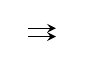
\begin{tikzpicture}[baseline]%
    \draw[>=stealth,->](0,0.15ex)--(\arrlen,0.15ex);%
    \draw[>=stealth,->](0,0.85ex)--(\arrlen,0.85ex);%
  \end{tikzpicture}}}
\newcommand{\lblto}[1]{\mathrel{%
    \begin{tikzpicture}[baseline= {( $ (current bounding box.south) + (0,-0.5ex) $ )}]
      \node[inner sep=.4ex] (a) {\,$\scriptstyle #1$\,};
      \draw[>=stealth,->] (a.south west) -- (a.south east);
    \end{tikzpicture}}}
\newcommand{\isoto}{\lblto{\sim}}

\newcommand{\simpl}[3]{
  \begin{tikzcd}[ampersand replacement=\&, column sep=small]
    #1 \&
    #2 \ar[l, shift right=0.35ex]
       \ar[l, shift left=0.35ex] \&
    #3 \ar[l, shift right=0.70ex]
       \ar[l, shift left=0.70ex]
       \ar[l] \&
    \cdots \ar[l, shift right=0.35ex]
           \ar[l, shift left=0.35ex]
           \ar[l, shift right=1.05ex]
           \ar[l, shift left=1.05ex]
  \end{tikzcd}
}
\newcommand{\cosimpl}[3]{
  \begin{tikzcd}[ampersand replacement=\&, column sep=small]
    #1 \ar[r, shift right=0.35ex]
       \ar[r, shift left=0.35ex] \&
    #2 \ar[r, shift right=0.70ex]
       \ar[r, shift left=0.70ex]
       \ar[r] \&
    #3 \ar[r, shift right=0.35ex]
       \ar[r, shift left=0.35ex]
       \ar[r, shift right=1.05ex]
       \ar[r, shift left=1.05ex] \&
    \cdots
  \end{tikzcd}
}

\newcommand{\tto}{\mathrel{\tikz[baseline]%
    \draw[>=stealth,->,double, double distance = 0.3ex](0,0.5ex)--(\arrlen,0.5ex);}}
\newcommand{\doubfrom}{\mathrel{%
  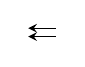
\begin{tikzpicture}[baseline]%
    \draw[>=stealth,<-](0,0.15ex)--(\arrlen,0.15ex);%
    \draw[>=stealth,<-](0,0.85ex)--(\arrlen,0.85ex);%
  \end{tikzpicture}}}
\newcommand{\tripfrom}{\mathrel{%
  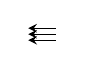
\begin{tikzpicture}[baseline]%
    \draw[>=stealth,<-](0,0.00ex)--(\arrlen,0.00ex);%
    \draw[>=stealth,<-](0,0.50ex)--(\arrlen,0.50ex);%
    \draw[>=stealth,<-](0,1.00ex)--(\arrlen,1.00ex);%
  \end{tikzpicture}}}


\renewcommand{\l}{\left}
\renewcommand{\r}{\right}
\newcommand{\f}{\frac}
\renewcommand{\o}{\overline}
\renewcommand{\u}{\underline}
\newcommand{\til}{\widetilde}
\renewcommand{\hat}{\widehat}
\newcommand{\del}{\partial}
\newcommand{\dash}{\text{-}}
\renewcommand{\c}{\colon}
\newcommand{\lc}{\,:\!}
\newcommand{\ce}{\coloneq}%{\mathrel{:=}}
\newcommand{\ec}{\eqcolon}%{\mathrel{=:}}
\newcommand{\iso}{\simeq}
\newcommand{\dual}{\vee}
\newcommand{\ldb}{\llbracket}
\newcommand{\rdb}{\rrbracket}

\newcommand{\Obj}{\operatorname{Obj}}
\newcommand{\Hom}{\operatorname{Hom}}
\newcommand{\Map}{\operatorname{Map}}
\newcommand{\Fun}{\operatorname{Fun}}
\newcommand{\Aut}{\operatorname{Aut}}
\newcommand{\Iso}{\operatorname{Iso}}
\renewcommand{\id}{\mathrm{id}}
\renewcommand{\im}{\operatorname{im}}
\newcommand{\op}{\mathrm{op}}
\newcommand{\univ}{\mathrm{univ}}
\newcommand{\colim}{\operatorname*{colim}}
\newcommand{\dlim}{\displaystyle\lim}
\newcommand{\dcolim}{\displaystyle\colim}
\newcommand{\Spec}{\operatorname{Spec}}
\newcommand{\Spf}{\operatorname{Spf}}

%%%%%%%%%%%%%%%%%%%%%%%%%%%%%%%%%%%%%%%%%%%%%%%%%%%%%%%%%%%%%%%%%%%%%%


\title{Thom spectra}
\author{Arpon Raksit}
\date{January 14, 2016}

\numberwithin{equation}{section}

\begin{document}
\maketitle

\newcommand{\Mod}{\mathrm{Mod}}
\newcommand{\Line}{\mathrm{Line}}
\newcommand{\GL}{\operatorname{GL}}
\newcommand{\Spaces}{\mathrm{Spaces}}
\newcommand{\Spectra}{\mathrm{Spectra}}
\newcommand{\cofib}{\operatorname*{cofib}}

%%%%%%%%%%%%%%%%%%%%%%%%%%%%%%%%%%%%%%%%%%%%%%%%%%%%%%%%%%%%%%%%%%%%%%

\section{Thom spectra in general}

In this section we formulate the Thom spectrum and the Thom isomorphism very generally, following [ABGHR](//arxiv.org/pdf/1403.4325v1.pdf). In the following sections we show how this formulation recovers the more classical notions of Thom space associated to vector/sphere bundles.

\begin{notation}
  Let $R$ be an $\rE_1$-ring spectrum. We denote the $\infty$-category of (left or right, just pick one to use throughout) $R$-module spectra by $\Mod(R)$. We denote the maximal subgroupoid of $\Mod(R)$ containing $R$ by $\Line(R)$.
\end{notation}

\begin{definition}
  Define the space $\GL_1(R)$ by the pullback
  \[
    \GL_1(R) \ce \Omega^{\infty}R \times_{\pi_0 R} (\pi_0 R)^\times.
  \]
  Since $R$ is an $\rE_1$-ring, $\GL_1(R)$ is an $\rE_1$-space, i.e. an $\infty$-group, hence has a delooping $\rB\GL_1(R)$. We call $\GL_1(R)$ the \emph{group of units} of $R$.
\end{definition}

\begin{lemma}
  \label{gl1-equiv-line}
  There's an equivalence of $\infty$-groups $\Aut_{\Mod(R)}(R) \iso \GL_1(R)$, and hence an equivalence of $\infty$-groupoids/spaces $\Line(R) \iso \rB\GL_1(R)$.
\end{lemma}

\begin{definition}
  Define the \emph{Thom spectrum} functor
  \[
    \rM \c \Spaces_{/\rB\GL_1(R)} \to \Mod(R)
  \]
  by sending a map $f \c X \to \rB\GL_1(R)$ to the colimit
  \[
    \rM f \ce  \colim \l(
    X \lblto{f} \rB\GL_1(R) \iso \Line(R) \inj \Mod(R) \r).
  \]
\end{definition}

%%%%%%%%%%%%%%%%%%%%%%%%%%%%%%%%%%%%%%%%%%%%%%%%%%%%%%%%%%%%%%%%%%%%%%

\section{Thom spectra of pointed sphere bundles}
\label{thom-ptd-sphere}

Our first stop on the way from the general Thom spectrum functor to Thom spectra of vector bundles is essentially to understand a part of the case when $R$ is the sphere spectrum.

\begin{definition}
  \label{ptd-sphere-bundle}
  A \label{pointed sphere bundle} of dimension $n \in \lZ_{\ge 0}$ over a space $X$ is a pair $(f, s)$ where
  \begin{enumerate}
  \item $f$ is a map of spaces $E \to X$ such that for every
    $x \in X$ the (homotopy) fiber $E_x$ is equivalent to the sphere
    $\rS^n$;
  \item $s$ is a section $X \to E$ of $f$.
  \end{enumerate}
\end{definition}

\begin{definition}
  \label{thom-spectrum-ptd-sphere}
  Let $(f \c E \to X, s \c X \to E)$ be a pointed sphere bundle of dimension $n \in \lZ_{\ge 0}$. We define the \emph{Thom space} $\o\rM f$ of $(f,s)$ to be the (homotopy) cofiber of $s$, i.e.
  \[
    \o\rM f \ce \cofib \l( X \lblto{s} E \r).
  \]
  We define the \emph{Thom spectrum} $\rM f$ of $(f,s)$ as the $n$-fold desuspension of the suspension spectrum of the Thom space $\o\rM f$, i.e.
  \[
    \rM f \ce \Sigma^{\infty - n} \o\rM f.
  \]
\end{definition}

\begin{notation}
  \label{sphere-spectrum}
  Let $\rS \ce \Sigma^\infty\rS^0$ denote the sphere spectrum. Recall that $\Mod(\rS)$ is just the $\infty$-category $\Spectra$ of spectra.
\end{notation}

\begin{definition}
  \label{stable-spherical-fibration}
  A \emph{stable sphere bundle} over a space $X$ is a functor $X \to \rB\GL_1(\rS)$.
\end{definition}

\begin{lemma}
  \label{gl1-sphere}
  There's an equivalence of $\infty$-groups
  \[
    \colim_{n \in \lZ_{\ge 0}} \Aut_{\Spaces_*}(\rS^n) \isoto
    \GL_1(\rS)
  \]
  induced by the maps $\Aut_{\Spaces_*}(\rS^n) \to \GL_1(\rS)$ sending a map $f \c \rS^n \to \rS^n$ to the map $\Sigma^{\infty - n}f \c \rS \to \rS$ in $\Aut_{\Spectra}(\rS)$, which is equivalent to $\GL_1(\rS)$ by @gl1-equiv-line.

  This induces an equivalence of $\infty$-groupoids
  \[
    \colim_{n \in \lZ_{\ge 0}} \rB\Aut_{\Spaces_*}(\rS^n) \iso
    \rB\GL_1(\rS).
  \]
\end{lemma}

\begin{construction}
  \label{ptd-sphere-to-stable-sphere}
  Here we associate to any pointed sphere bundle over $X$ a stable sphere bundle over $X$.

  Let $(f \c E \to X, s \c X \to E)$ be a pointed sphere bundle of dimension $n \in \lZ_{\ge 0}$. By the Grothendieck construction this data is equivalent to a functor $X \to \Spaces_*$ factoring through the maximal subgroupoid of $\Spaces_*$ containing $\rS^n$ (equipped with some chosen basepoint), i.e. a functor/map $F \c X \to \rB\Aut_{\Spaces_*}(\rS^n)$. As stated in @gl1-sphere there's a canonical map $\rB\Aut_{\Spaces_*}(\rS^n) \to \rB\GL_1(\rS)$; composing $F$ with this map gives us the desired stable sphere bundle $X \to \rB\GL_1(\rS)$.
\end{construction}

\begin{lemma}
  \label{thom-ptd-sphere-agrees}
  Let $(f \c E \to X, s \c X \to E)$ be a pointed sphere bundle of dimension $n \in \lZ_{\ge 0}$. Let $g \c X \to \rB\GL_1(\rS)$ be the associated stable sphere bundle constructed in @ptd-sphere-to-stable-sphere. Then our two definitions of Thom spectrum agree: $\rM f \iso \rM g$.
\end{lemma}

\begin{proof}
  Consider the diagram of functors
  \[
    \begin{tikzcd}
      \Fun(X, \rB\Aut_{\Spaces_*}(\rS^n)) \ar[d] \ar[r] &
      \Fun(X, \Spaces_*) \ar[d, "\Sigma^{\infty - n}"] \ar[r, "\colim"] &
      \Spaces_* \ar[d, "\Sigma^{\infty - n}"] \\
      \Fun(X, \rB\GL_1(\rS)) \ar[r] &
      \Fun(X, \Spectra) \ar[r, "\colim"] &
      \Spectra.
    \end{tikzcd}
  \]
  The left-hand square commutes by the definition (see @gl1-sphere) of the map $\rB\Aut_{\Spaces_*}(\rS^n) \to \rB\GL_1(\rS)$ inducing the left-hand vertical arrow. The right-hand square commutes because $\Sigma^\infty$ is a left-adjoint and hence commutes with colimits. Hence the whole diagram commutes. Now, via the Grothendieck construction the composite of the top row can be identified with the Thom space construction for pointed sphere bundles $(f,s) \mapsto \o\rM f$, whence going around the diagram clockwise gives the Thom spectrum $\rM f$. On the other hand going around the diagram counter-clockwise gives the Thom spectrum $\rM g$, finishing the proof.
\end{proof}

%%%%%%%%%%%%%%%%%%%%%%%%%%%%%%%%%%%%%%%%%%%%%%%%%%%%%%%%%%%%%%%%%%%%%%

\section{Thom spectra of sphere bundles}
\label{thom-sphere}

Here's an alternate take on @thom-ptd-sphere where instead of requiring pointedness built into our sphere bundles we install it ourselves manually via a suspension. (We'll see below that this amounts in the case of vector bundles to considering the unit sphere sub-bundle instead of the fiberwise one-point compactification.)

\begin{definition}
  \label{sphere-bundle}
  A \emph{sphere bundle} of dimension $n \in \lZ_{\ge 0}$ over a space $X$ is a map of spaces $E \to X$ such that for every $x \in X$ the (homotopy) fiber $E_x$ is equivalent to the sphere $\rS^n$.
\end{definition}

\begin{definition}
  \label{thom-spectrum-sphere}
  Let $f \c E \to X$ be a sphere bundle of dimension $n \in \lZ_{\ge 1}$. We define the \emph{Thom space} $\o\rM f$ of $f$ to be the (homotopy) cofiber of $f$, i.e.
  \[
    \o\rM f \ce \cofib \l( E \lblto{f} X \r).
  \]
  We define the \emph{Thom spectrum} $\rM f$ of $f$ as the $(n+1)$-fold desuspension of the suspension spectrum of the Thom space $\o\rM f$, i.e.
  \[
    \rM f \ce \Sigma^{\infty - n-1} \o\rM f.
  \]
\end{definition}

\begin{construction}
  \label{sphere-to-ptd-sphere}
  Here we associate to any sphere bundle $f \c E \to X$ of dimension $n \in \lZ_{\ge 0}$ a pointed sphere bundle of dimension $n+1$ over $X$.

  By the Grothendieck construction we identify $f$ with a functor $X \to \Spaces$ factoring through the maximal subgroupoid $\rB\Aut_{\Spaces}(\rS^n)$ of $\Spaces$ containing $\rS^n$. Composing with the suspension functor $\Sigma \c \Spaces \to \Spaces_*$ (where we take the basepoint to be the top of the suspension, say) gives us a functor $X \to \Spaces_*$ factoring through the maximal subgroupoid $\rB\Aut_{\Spaces_*}(\rS^{n+1})$ containing $\rS^{n+1}$, and again by the Grothendieck construction this is the pointed sphere bundle of dimension $n+1$ we wanted.
\end{construction}

\begin{lemma}
  \label{thom-sphere-agrees}
  Let $f \c E \to X$ be a sphere bundle of dimension $n \in \lZ_{\ge 0}$. Let $(g \c E' \to X, s \c X \to E')$ be the associated pointed sphere bundle of dimension $n+1$ constructed in @sphere-to-ptd-sphere. Then our two definitions of Thom space agree: $\o\rM f \iso \o\rM g$. It follows immediately that the Thom spectra agree as well: $\rM f \iso \rM g$.
\end{lemma}

\begin{proof}
  Consider the diagram of functors
  \[
    \begin{tikzcd}
      \Fun(X, \rB\Aut_{\Spaces}(\rS^n)) \ar[d] \ar[r] &
      \Fun(X, \Spaces) \ar[d, "\Sigma \iso \cofib(- \to *)"] \ar[r, "\colim"] &
      \Spaces_{/X} \ar[d, "\cofib"] \\
      \Fun(X, \rB\Aut_{\Spaces_*}(\rS^{n+1})) \ar[r] &
      \Fun(X, \Spaces_*) \ar[r, "\colim"] &
      \Spaces_*.
    \end{tikzcd}
  \]
  The left-hand square commutes by the definition (see @sphere-to-ptd-sphere) of the map $\rB\Aut_{\Spaces}(\rS^n) \to rB\Aut_{\Spaces_*}(\rS^{n+1})$ inducing the left-hand vertical arrow. The right-hand square commutes because colimits commute with cofibers. Hence the whole diagram commutes. Now, the top-right horizontal map is the Grothendieck construction, whence going around the diagram clockwise gives the Thom space $\o\rM f$. On the other hand, as in the proof of @thom-ptd-sphere-agrees, going around the diagram counter-clockwise gives the Thom space $\o\rM g$, finishing the proof.
\end{proof}

% \bibliographystyle{amsalpha}
% \bibliography{refs}

\end{document}
